\documentclass[a4paper, 11pt]{article}

% Added by us
\usepackage{graphicx}
\usepackage{cleveref}
\usepackage{caption}
\usepackage{float}
\usepackage{multicol}
\usepackage{makecell}
\usepackage{array}
\usepackage{color, colortbl}
\usepackage{xr}
\newcolumntype{P}[1]{>{\centering\arraybackslash}m{#1}}
% \renewrobustcmd{\bfseries}{\fontseries{b}\selectfont}
% \renewrobustcmd{\boldmath}{}
% \newrobustcmd{\B}{\bfseries}

\newcommand{\dieuwke}[1]{\textcolor{blue}{DH: #1}}
\newcommand{\beginsupplement}{%
        \setcounter{table}{0}
        \renewcommand{\thetable}{S\arabic{table}}%
        \setcounter{figure}{0}
        \renewcommand{\thefigure}{S\arabic{figure}}%
     }

\begin{document}
\beginsupplement

\begin{figure}
    \centering
    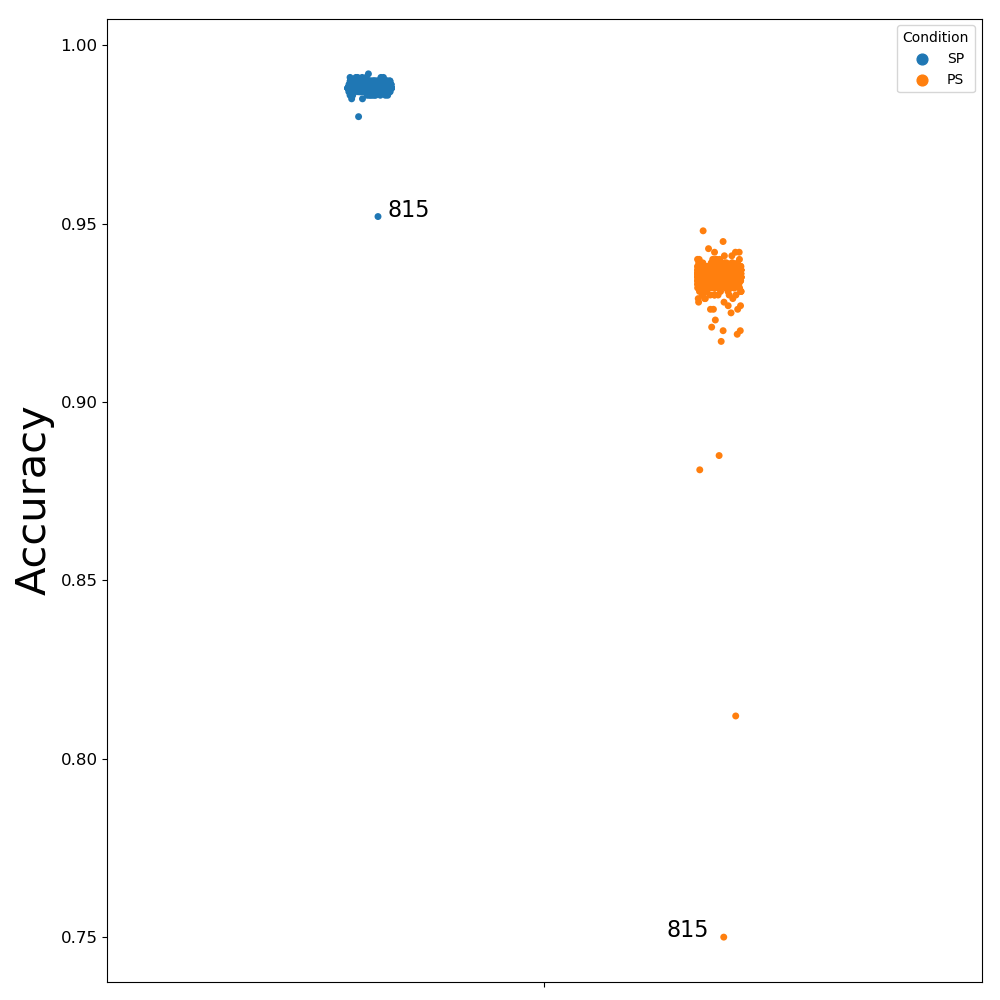
\includegraphics[width=10cm]{figures/Ablation_results_K_model.png}
    \caption{\textbf{Ablation results for the model from Gulordave et. al, 2018}}
    \label{fig:ablation_K_model}
\end{figure}

\begin{figure}
    \centering
    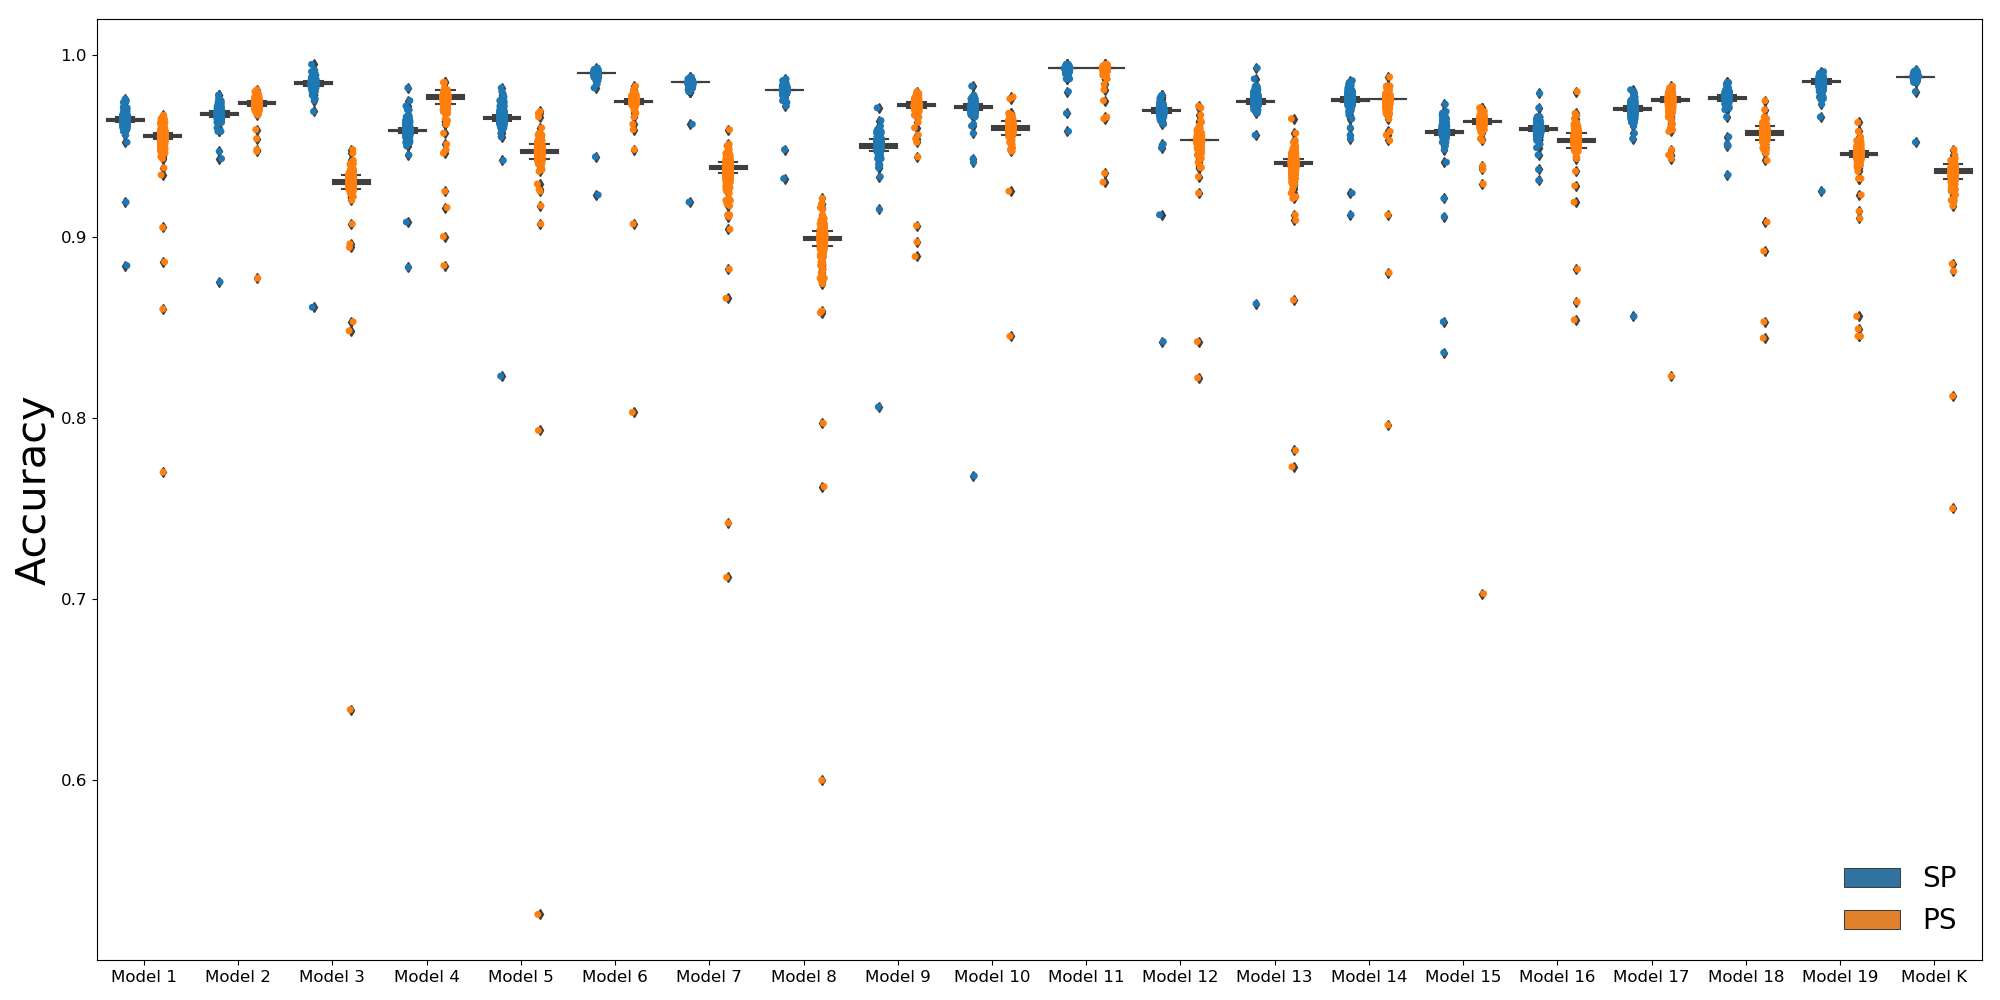
\includegraphics[width=15cm]{figures/Ablation_results_all_models.png}
    \caption{\textbf{Ablation results for all 20 models}}
    \label{fig:ablation_all_models}
\end{figure}


\begin{figure}[h]
    \centering
    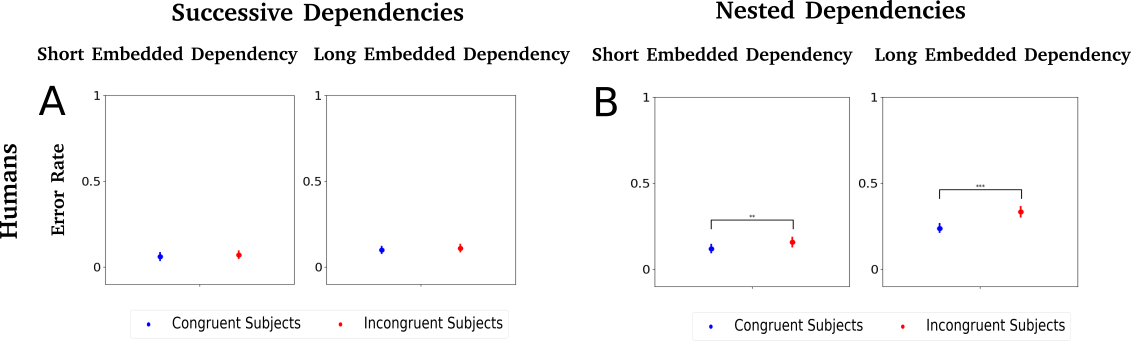
\includegraphics[width=16cm]{figures/error_rates_acceptable_by_congruence.png}
    \caption{\textbf{Error rates on grammatical sentences:} for successive (panel A) and nested dependencies (B). Blue and red correspond to whether the main and embedded subjects agree on number (congruent subjects) or not (incongruent), respectively. Error bars represent standard error of the mean across all trials.}
    \label{fig:error_rates_all_conditions}
\end{figure}

% \begin{center}
\begin{table}
\centering
\begin{tabular}{|P{3.3cm}|P{2.5cm}|P{1.2cm}|P{1.5cm}|P{1.5cm}|P{1.3cm}|P{1.5cm}|P{1.5cm}|}
    \hline
    \multicolumn{1}{|c|}{\B Task} & \multicolumn{1}{|c|}{\B Verb} & \multicolumn{3}{|c|}{\B Humans} & \multicolumn{3}{|c|}{\B NLM}\\
    \hline
    \B & \B  & \B $\beta$ & \B z-score & \B p-value & \B $\beta$ & \B z-score & \B p-value\\
    \hline
    \B Successive-Short & \B Embedded & -0.904 & -1.810 & 0.070 & -18.31 & -0.012 & 0.990 \\
    \hline
    \B Successive-Long & \B Embedded  & 0.114 & 0.475 & 0.635 & -2.190 & -4.615 & \B <0.001 \\
    \hline
    \B Nested-Short & \B Main & 0.535 & 2.210 & \B 0.027 & -0.147 & -1.239 & 0.215\\
    \hline
    \B Nested-Short & \B Embedded  & 0.470 & 2.429 & \B 0.015 & -0.481 & -5.252 & \B <0.001 \\
    \hline
    \B Nested-Long & \B Main & 0.244 & 1.684 & 0.092 & -1.2442 & -10.038  & \B <0.001 \\
    \hline
    \B Nested-Long & \B Embedded  & 0.890 & 6.585 & \B <0.001 & -0.542 & -3.579 & \B < 0.001\\
    \hline
\end{tabular}
\caption{\textbf{Effects of grammatical number for humans and the NLM}: for each number-agreement task and each verb, we fitted a logistic regression model with subject-congruence and grammatical number of the attractor subject as variables. In the case of Long-Successive and Long-Nested, the model also included a variable for whether the attractor is congruent or not with the embedded subject. A positive $\beta$ means more errors due to a plural attractor. Significant p-values (<0.05) are marked in bold. }
\label{tbl:stats_number}
\end{table}
\end{center}

\section{Lexicon NA-tasks}\ref{appendix:lexicon}

\dieuwke{Include here the lexicon of the NA-tasks}

\end{document}
